\newsavebox{\hmmtikzpicture}
\sbox{\hmmtikzpicture}{%
	\tikzset{external/export next=false}%
% use these distances to manipulate the size
\let\hmmhdist\relax % avoid errors if lenght is already existing
\let\hmmvdist\relax % avoid errors if lenght is already existing
\newlength{\hmmhdist}%
\newlength{\hmmvdist}%
\setlength{\hmmhdist}{.8em}%
\setlength{\hmmvdist}{.5em}%
\begin{tikzpicture}
	\tikzstyle{state}=[%
	circle,
	thin,
	minimum size=1.2em,
	inner sep=.1em,
	outer sep=.1em,
	draw=primary_inverse_fg,
	fill=primary_inverse_bg,
	text=primary_inverse_fg,
	font=\tiny
	]
	\tikzstyle{match}=[state, rectangle]
	\tikzstyle{insert}=[state, diamond]
	\tikzstyle{be}=[%
	state,
	draw=primary_accent_fg,
	fill=primary_accent_bg,
	text=primary_accent_fg
	]
	\tikzstyle{delete}=[state]
	\tikzstyle{transition}=[%
	ultra thin,
	-{Latex[width=1mm,length=1mm]},
	primary_inverse_fg
	]
	\tikzstyle{every loop}=[transition, min distance=0em, looseness=2mm]
	\node [be] (b) {$B$};
	\node [match, right=\hmmhdist of b] (m1) {$M_1$};
	\node [match, right=\hmmhdist of m1] (m2) {$M_2$};
	\node [match, right=\hmmhdist of m2] (m3) {$M_3$};
	\node [be, right=\hmmhdist of m3] (e) {$E$};
	\coordinate (mb1) at ($(b.north)!0.5!(m1.north)$);
	\coordinate (m12) at ($(m1.north)!0.5!(m2.north)$);
	\coordinate (m23) at ($(m2.north)!0.5!(m3.north)$);
	\coordinate (m3e) at ($(m3.north)!0.5!(e.north)$);
	\node [insert, above=\hmmvdist of mb1] (i0) {$I_0$};
	\node [insert, above=\hmmvdist of m12] (i1) {$I_1$};
	\node [insert, above=\hmmvdist of m23] (i2) {$I_2$};
	\node [insert, above=\hmmvdist of m3e] (i3) {$I_3$};
	\node [delete, below=\hmmvdist of m1] (d1) {$D_1$};
	\node [delete, below=\hmmvdist of m2] (d2) {$D_2$};
	\node [delete, below=\hmmvdist of m3] (d3) {$D_3$};
	\draw [transition] (b) -- (m1);
	\draw [transition] (b) -- (i0);
	\draw [transition] (b) -- (d1);
	\draw [transition] (m1) -- (m2);
	\draw [transition] (m2) -- (m3);
	\draw [transition] (m3) -- (e);
	\draw [transition] (m1) -- (i1);
	\draw [transition] (m2) -- (i2);
	\draw [transition] (m3) -- (i3);
	\draw [transition] (i0) -- (m1);
	\draw [transition] (i1) -- (m2);
	\draw [transition] (i2) -- (m3);
	\draw [transition] (i3) -- (e);
	\draw [transition] (d1) -- (d2);
	\draw [transition] (d2) -- (d3);
	\draw [transition] (d3) -- (e);
	\draw [transition] (m1) -- (d2);
	\draw [transition] (m2) -- (d3);
	\draw [transition] (d1) -- (m2);
	\draw [transition] (d2) -- (m3);
	\draw (i0) edge [loop above] ();
	\draw (i1) edge [loop above] ();
	\draw (i2) edge [loop above] ();
	\draw (i3) edge [loop above] ();
\end{tikzpicture}%
%
}
\newsavebox{\mutidtikzpicture}
\sbox{\mutidtikzpicture}{%
	\tikzset{external/export next=false}%
\begin{tikzpicture}
	\tikzstyle{every node}=[%
	object,
	inner sep=.3em,
	outer sep=.4em,
	text width=2em,
	minimum height=.5em,
	font=\footnotesize,
	fill=primary_accent_bg,
	text=primary_accent_fg
	]
	\node (S) {Ser};
	\node [right=1.2em of S] (T) {Thr};
	\draw [->, draw=primary_inverse_fg] (S) -- (T);
\end{tikzpicture}%
%
}
\tikzset{external/export next=false}%
\begin{tikzpicture}
	\node [object, text width=8em, minimum height=6em, text depth=4em] (a) {%
		Mutation identity
		\vspace{1.7em}
		\begin{figure}\usebox{\mutidtikzpicture}\vfill\end{figure}
	};
	%\node [object, below=-.3em of a, font=\tiny, text width=8em] (a1) {\sbseries Wild-type residue};
	%\node [object, below=-.3em of a1, font=\tiny, text width=8em] (a2) {\sbseries Mutated residue};
	\node [object, right=2em of a, text width=8em, minimum height=6em] (b) {%
	EVmutation predictions\\{\tiny\parencite{Hopf2017}}
	\vspace{1em}
	\begin{figure}
		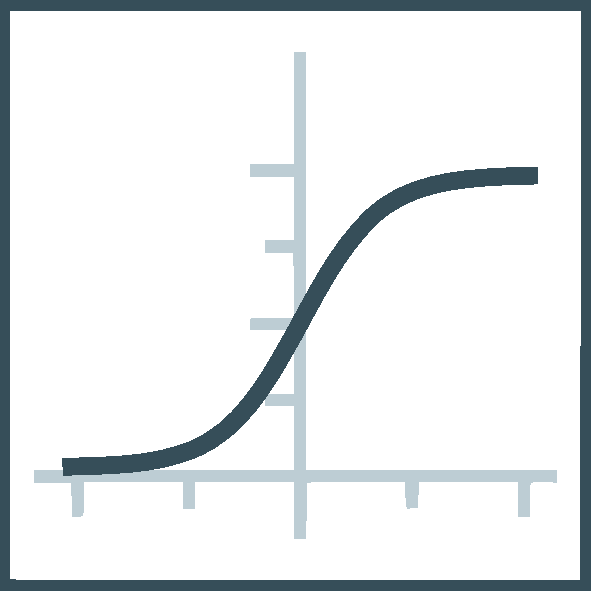
\includegraphics[height=3em]{images/sigmoid.pdf}
	\end{figure}
	};
	%\node [object, below=-.3em of b, font=\tiny, text width=8em] (b1) {\sbseries Epistatic model};
	%\node [object, below=-.3em of b1, font=\tiny, text width=8em] (b2) {\sbseries Independent model};
	%\node [object, below=-.3em of b2, font=\tiny, text width=8em] (b3) {\sbseries Conservation};
	%\node [object, below=-.3em of b3, font=\tiny, text width=8em] (b4) {\sbseries Mutation frequency};
	\node [object, right=2em of b, text width=8em, minimum height=6em] (c) {%
	NetsurfP-2 predictions\\{\tiny\parencite{Klausen2019}}
	\vspace{1em}
	\begin{figure}
		
\includegraphics[height=3em]{images/ai.pdf}
	\end{figure}
	};
	%\node [object, below=-.3em of netsurf, font=\tiny, text width=8em] (sec) {\sbseries Secondary structure};
	%\node [object, below=-.3em of sec, font=\tiny, text width=8em] (rsa) {\sbseries Solvent accessibility};
	%\node [object, below=-.3em of rsa, font=\tiny, text width=8em] (dis) {\sbseries Disorder};
	%\node [object, below=-.3em of dis, font=\tiny, text width=8em] (tors) {\sbseries Torsion angles};
	\node [object, below=1em of b, text width=13em, xshift=-8em, minimum height=10em] (d) {%
	HMMER emission probabilities\\{\tiny\parencite{Eddy2011}}
	\vspace{1em}
	\begin{figure}\usebox{\hmmtikzpicture}\end{figure}
	};
	\node [object, below=1em of b, text width=13em, xshift=8em, minimum height=10em, text depth=8.1em] (e) {%
	trRosetta predicted contacts\\{\tiny\parencite{Yang2020}}
	\vspace{1.5em}
	\begin{figure}
		
\includegraphics[height=7em]{images/ai.pdf}
	\end{figure}

	};
	%\node [object, below=-.3em of e, font=\tiny, text width=13em] (e1) {\sbseries Centrality metrics};
\end{tikzpicture}%
